\chapter{Décrire un système chimique~: avancement, activités, Q et K}\label{ch:b1:extent-q-and-k}

Une usine à hydrogène fait passer du gaz naturel et de la vapeur d'eau
dans des tubes chauffés au rouge~; il n'en sort jamais du dihydrogène
pur, mais un mélange de dihydrogène, de monoxyde de carbone, de dioxyde
de carbone, de méthane n'ayant pas réagi et de vapeur d'eau, dont les
ingénieurs doivent connaître les proportions avant de dimensionner
l'unité suivante. Prévoir la composition qui sort d'un réacteur --- l'état
final d'un système chimique --- est l'objet de ce chapitre. Il faut pour
cela une description précise du système (ses variables et sa
composition), un nombre unique qui mesure jusqu'où une réaction est
allée (l'\omterm{def:b1:extent-q-and-k:extent}{avancement}), et la loi qui dit où la réaction s'arrête (la
constante d'équilibre). Ces outils servent dans tous les chapitres
suivants sur les solutions.

\begin{recall}
Le livre 1 (année 10) a suivi une réaction à l'aide d'un tableau
d'\omterm{def:b1:extent-q-and-k:extent}{avancement} et déterminé le \omterm{def:b1:extent-q-and-k:max-extent}{réactif limitant}~; le livre 1 (année 12) a
introduit le \omterm{def:b1:extent-q-and-k:quotient}{quotient de réaction} $Q$ et la constante d'équilibre $K$
d'une réaction non totale. On utilise, comme acquise en physique, la loi
des gaz parfaits $pV = nRT$, avec $R =
\qty{8.314}{J/(mol.K)}$.
\end{recall}

\begin{omfigure}
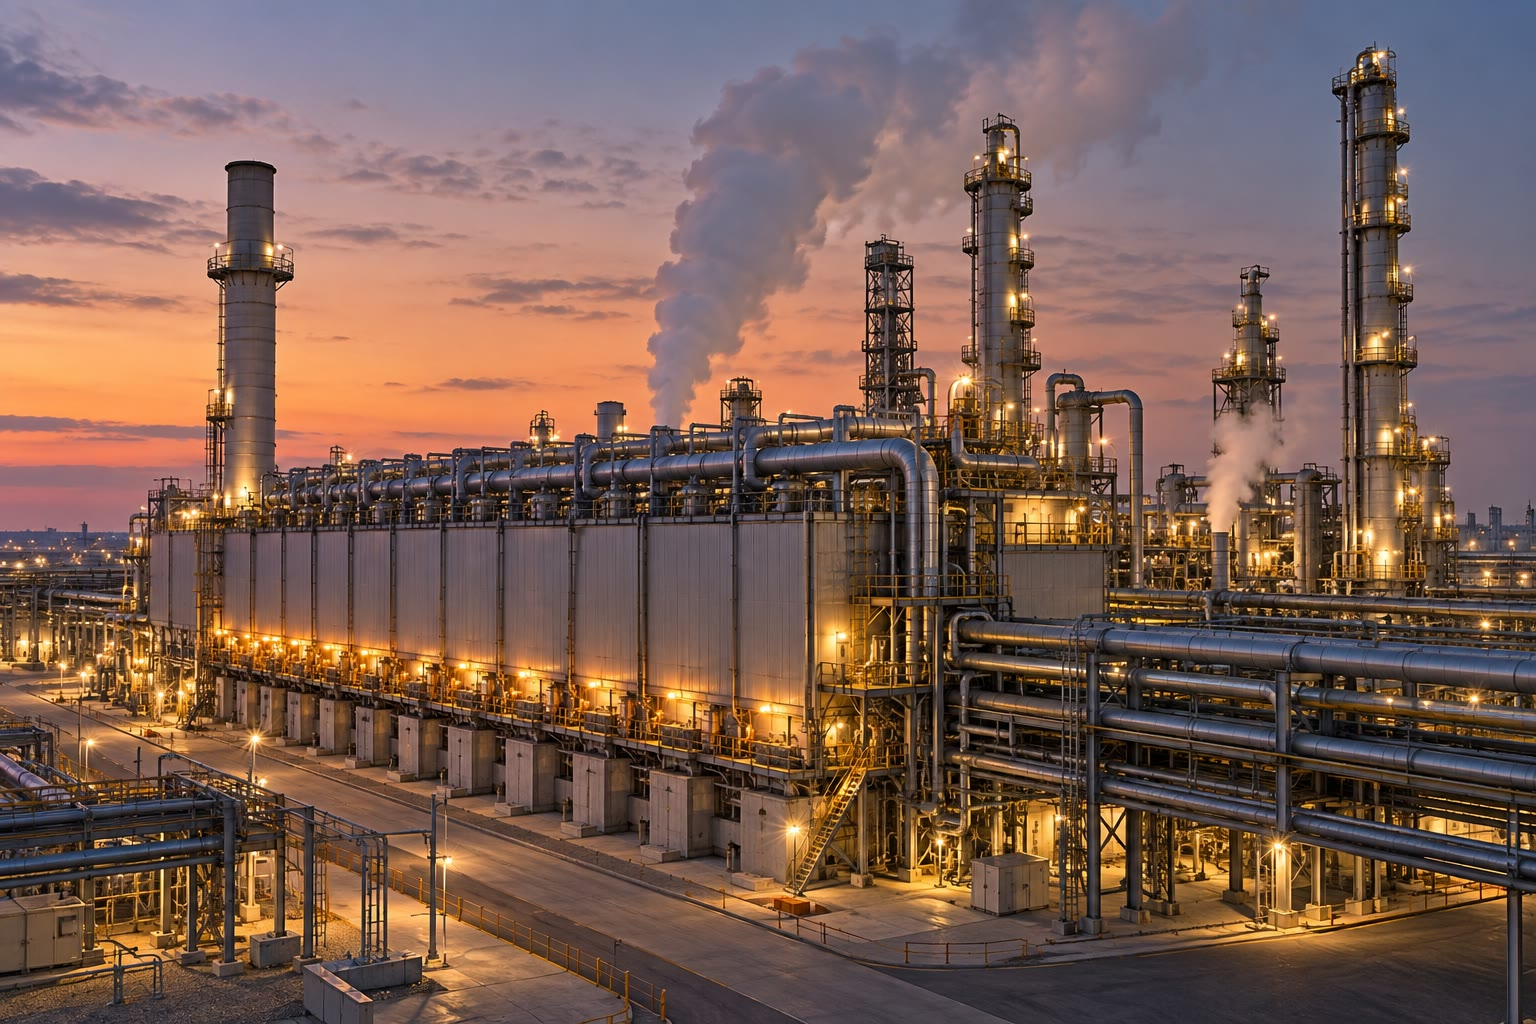
\includegraphics[width=0.6\linewidth]{images/book2/ai/b1-07-hydrogen-plant.jpg}

{\small Une usine à hydrogène au crépuscule. Le gaz naturel et la vapeur
d'eau réagissent dans le long four de reformage~; un second réacteur
convertit le monoxyde de carbone~; la composition en sortie est un état
final du type calculé dans ce chapitre.}
\end{omfigure}

\section{Décrire un système}

\begin{definition}[Système, phase]\label{def:b1:extent-q-and-k:system}
Un \emph{système physico-chimique}\index{systeme physico-chimique@système physico-chimique} est la matière
contenue dans une région de l'espace choisie, le reste constituant le
milieu extérieur. C'est un \emph{système fermé}\index{systeme ferme@système fermé} s'il
n'échange pas de matière avec l'extérieur (il peut échanger de
l'énergie). Une \emph{phase}\index{phase} est une partie du système dans
laquelle les \omterm{def:b1:extent-q-and-k:variables}{variables intensives} varient de façon continue~: un
mélange gazeux forme une seule phase, deux liquides non \omterm{def:b1:intermolecular-forces-solvents:miscibility}{miscibles}
forment deux phases, chaque solide est une phase à lui seul.
\end{definition}

\begin{definition}[Variables intensives et extensives]\label{def:b1:extent-q-and-k:variables}
Une variable d'état est \emph{extensive}\index{variable extensive} si elle
est proportionnelle à la taille du système (masse, volume, quantité de
matière) et \emph{intensive}\index{variable intensive} sinon
(température, pression, concentration, masse volumique, \omterm{def:b1:extent-q-and-k:composition}{fraction
molaire}). Le rapport de deux variables extensives est intensif.
\end{definition}

\begin{definition}[Variables de composition]\label{def:b1:extent-q-and-k:composition}
Pour un constituant $i$ d'une \omterm{def:b1:extent-q-and-k:system}{phase} qui contient les quantités $n_j$ de
tous ses constituants~:
\begin{itemize}
  \item sa \emph{fraction molaire}\index{fraction molaire} est $x_i = n_i/\sum_j
        n_j$, et sa \emph{fraction massique}\index{fraction massique} $w_i =
        m_i/\sum_j m_j$~; toutes deux sont comprises entre 0 et 1 et ont
        pour somme 1~;
  \item dans une solution de volume $V$, sa \emph{concentration
        molaire}\index{concentration molaire} est $c_i = [i] = n_i/V$,
        en \unit{mol/L}~;
  \item dans un mélange gazeux sous la pression totale $p$, sa
        \emph{pression partielle}\index{pression partielle} est $p_i = x_i\,p$.
\end{itemize}
\end{definition}

\begin{proposition}[Pressions partielles des gaz parfaits]\label{prop:b1:extent-q-and-k:dalton}
Dans un mélange de gaz parfaits de volume $V$ à la température $T$, la
\omterm{def:b1:extent-q-and-k:composition}{pression partielle} d'un constituant est la pression qu'il exercerait
s'il occupait seul tout le volume, $p_i = n_iRT/V$, et la somme des
\omterm{def:b1:extent-q-and-k:composition}{pressions partielles} est la pression totale~: $\sum_i p_i = p$.
\end{proposition}

\begin{proof}
Pour le mélange, $pV = (\sum_j n_j)RT$, donc $p_i = x_i p = \frac{n_i}{\sum_j
n_j}\cdot\frac{(\sum_j n_j)RT}{V} = \frac{n_iRT}{V}$, et $\sum_i x_i = 1$
donne $\sum_i p_i = p$.
\end{proof}

\begin{example}[L'air]\label{ex:b1:extent-q-and-k:air}
L'air sec contient, en volume (c'est-à-dire en quantité de matière, pour
des gaz parfaits), 78.08\,\% de diazote, 20.95\,\% de dioxygène et
0.93\,\% d'argon. Sous \qty{1.013}{bar}, la \omterm{def:b1:extent-q-and-k:composition}{pression partielle} du
dioxygène vaut $0.2095 \times
1.013 = \qty{0.212}{bar}$~; en montagne, là où la pression vaut
\qty{0.70}{bar}, elle tombe à \qty{0.147}{bar}, bien que la composition
soit la même.
% ledger: air:N2, air:O2, air:Ar, const:atm
\end{example}

\section{Avancement d'une réaction}

\begin{definition}[Nombres stœchiométriques, avancement]\label{def:b1:extent-q-and-k:extent}
Une réaction s'écrit $0 = \sum_i \nu_i\,\mathrm{A}_i$, où le
\emph{nombre stœchiométrique}\index{nombre stoechiometrique@nombre stœchiométrique} $\nu_i$ de l'espèce
$\mathrm{A}_i$ est négatif pour un réactif et positif pour un produit~:
dans \ce{N2 + 3H2 -> 2NH3}, $\nu(\ce{N2}) = -1$, $\nu(\ce{H2}) = -3$,
$\nu(\ce{NH3}) = +2$. Dans un \omterm{def:b1:extent-q-and-k:system}{système fermé} siège de cette seule
réaction, les quantités évoluent selon
\[
  n_i = n_{i,0} + \nu_i\,\xi ,
\]
ce qui définit l'\emph{avancement}\index{avancement} de la réaction
$\xi$ (en moles), nul au départ et le même pour toutes les espèces.
\end{definition}

\begin{definition}[Avancement maximal, réactif limitant]\label{def:b1:extent-q-and-k:max-extent}
L'\emph{avancement maximal}\index{avancement maximal} $\xi_{\max}$ est la plus grande
valeur de $\xi$ pour laquelle aucune quantité n'est négative~: $\xi_{\max} = \min_{\nu_i <
0} n_{i,0}/|\nu_i|$. Le réactif dont la quantité s'annule en $\xi_{\max}$
est le \emph{réactif limitant}\index{reactif limitant@réactif limitant}. Lorsque l'\omterm{def:b1:extent-q-and-k:extent}{avancement} peut
aussi être négatif (réaction en sens inverse), $\xi_{\min} = -\min_{\nu_i > 0}
n_{i,0}/\nu_i$.
\end{definition}

\begin{method}[Le tableau d'avancement]\label{met:b1:extent-q-and-k:progress-table}
Pour suivre une réaction dans un \omterm{def:b1:extent-q-and-k:system}{système fermé}~:
\begin{enumerate}
  \item écrire l'équation ajustée et, au-dessous, une colonne par espèce~;
  \item première ligne~: les quantités initiales $n_{i,0}$~;
  \item deuxième ligne~: les quantités à l'\omterm{def:b1:extent-q-and-k:extent}{avancement} $\xi$, $n_{i,0} + \nu_i\xi$~;
  \item pour des gaz, ajouter une colonne donnant la quantité totale
        $n_{\text{tot}}(\xi)$~;
  \item calculer $\xi_{\max}$ (et $\xi_{\min}$) et identifier le \omterm{def:b1:extent-q-and-k:max-extent}{réactif
        limitant}~;
  \item dernière ligne~: les quantités finales, à l'\omterm{def:b1:extent-q-and-k:extent}{avancement} final
        $\xi_f$ (déterminé par la condition d'équilibre, ou égal à
        $\xi_{\max}$ si la réaction est totale).
\end{enumerate}
\end{method}

\begin{example}[Synthèse de l'ammoniac]\label{ex:b1:extent-q-and-k:ammonia}
À partir de \qty{2.0}{mol} de \ce{N2} et de \qty{3.0}{mol} de \ce{H2}~:
\begin{center}
\begin{tabular}{lcccc}
\hline
 & \ce{N2} & \ce{3H2} & \ce{2NH3} & total \\
\hline
initial & 2.0 & 3.0 & 0 & 5.0 \\
\omterm{def:b1:extent-q-and-k:extent}{avancement} $\xi$ & $2.0 - \xi$ & $3.0 - 3\xi$ & $2\xi$ & $5.0 - 2\xi$ \\
\hline
\end{tabular}
\end{center}
$\xi_{\max} = \min(2.0/1,\ 3.0/3) = \qty{1.0}{mol}$~: le dihydrogène est
limitant. Si la réaction était totale, l'état final contiendrait
\qty{1.0}{mol} de \ce{N2} et \qty{2.0}{mol} de \ce{NH3}.
\end{example}

\begin{definition}[Taux d'avancement final, rendement]\label{def:b1:extent-q-and-k:fractional-extent}
Le \emph{taux d'avancement final}\index{taux d'avancement final} d'une
réaction est $\tau = \xi_f/\xi_{\max}$, compris entre 0 et 1. Dans une
synthèse, le \emph{rendement}\index{rendement} en un produit est le rapport
de la quantité obtenue à celle que donnerait le \omterm{def:b1:extent-q-and-k:max-extent}{réactif limitant} si la
réaction était totale~; lorsque le produit n'est pas perdu lors de
l'isolement, il est égal à $\tau$.
\end{definition}

\section{Activités}

\begin{definition}[État standard, activité]\label{def:b1:extent-q-and-k:activity}
L'\emph{activité}\index{activite@activité} $a_i$ d'une espèce est un nombre sans dimension
qui mesure, dans l'expression des lois d'équilibre, la quantité de
cette espèce effectivement disponible~; elle est définie par rapport à
un \emph{état standard}\index{etat standard@état standard}, état de référence à la
température considérée et sous la pression standard
$p^\circ = \qty{1}{bar}$. Dans les approximations idéales utilisées dans
ce livre~:
\begin{itemize}
  \item pour un gaz, $a_i = p_i/p^\circ$ (l'état standard est le gaz
        parfait pur sous $p^\circ$)~;
  \item pour un soluté en solution diluée, $a_i = c_i/c^\circ$ avec
        $c^\circ = \qty{1}{mol/L}$~;
  \item pour le solvant d'une solution diluée, et pour un solide pur ou
        un liquide pur seul dans sa \omterm{def:b1:extent-q-and-k:system}{phase}, $a_i = 1$.
\end{itemize}
\end{definition}
% ledger: const:pstd

\begin{remark}[Idéal et réel]\label{rem:b1:extent-q-and-k:ideal}
Ces expressions valent pour les gaz parfaits et les solutions diluées.
Dans les solutions concentrées, les ions s'attirent et se repoussent et
l'\omterm{def:b1:extent-q-and-k:activity}{activité} s'écarte de $c_i/c^\circ$~; les corrections, écrites à l'aide
de coefficients d'\omterm{def:b1:extent-q-and-k:activity}{activité}, sont étudiées dans le volume de deuxième
année avec le potentiel chimique. Pour les concentrations utilisées
dans ce livre (inférieures à \qty{0.1}{mol/L} environ), les expressions
idéales sont exactes à quelques pour cent près.
\end{remark}

\section{Le quotient de réaction et la constante d'équilibre}

\begin{definition}[Quotient de réaction]\label{def:b1:extent-q-and-k:quotient}
Le \emph{quotient de réaction}\index{quotient de reaction@quotient de réaction} d'une réaction
$0 = \sum_i \nu_i\,\mathrm{A}_i$ dans un état donné du système vaut
\[
  Q = \prod_i a_i^{\nu_i} ,
\]
le produit des \omterm{def:b1:extent-q-and-k:activity}{activités} des produits divisé par celui des \omterm{def:b1:extent-q-and-k:activity}{activités} des
réactifs, chacune élevée à la puissance de son coefficient
stœchiométrique.
\end{definition}

\begin{example}[Trois quotients]\label{ex:b1:extent-q-and-k:quotients}
Pour \ce{N2(g) + 3H2(g) <=> 2NH3(g)}~: $Q = \dfrac{(p_{\ce{NH3}}/p^\circ)^2}
{(p_{\ce{N2}}/p^\circ)(p_{\ce{H2}}/p^\circ)^3}$. Pour
\ce{CH3COOH(aq) + H2O(l) <=> CH3COO^-(aq) + H3O+(aq)}~: $Q =
\dfrac{[\ce{CH3COO-}][\ce{H3O+}]}{[\ce{CH3COOH}]\,c^\circ}$, le solvant
ayant une \omterm{def:b1:extent-q-and-k:activity}{activité} égale à 1. Pour \ce{CaCO3(s) <=> CaO(s) + CO2(g)}~:
$Q =
p_{\ce{CO2}}/p^\circ$, les solides ayant une \omterm{def:b1:extent-q-and-k:activity}{activité} égale à 1.
\end{example}

\begin{definition}[Constante d'équilibre standard]\label{def:b1:extent-q-and-k:equilibrium-constant}
La \emph{constante d'équilibre standard}\index{constante d'equilibre standard@constante d'équilibre standard}
$K^\circ$ d'une réaction est la valeur prise par son \omterm{def:b1:extent-q-and-k:quotient}{quotient de
réaction} lorsque le système est à l'équilibre. Elle est sans dimension et
ne dépend que de la réaction et de la température.
\end{definition}

\begin{theorem}[Loi d'action des masses]\label{thm:b1:extent-q-and-k:mass-action}
À une température donnée, un système siège d'une réaction possible dans
les deux sens évolue jusqu'à ce que $Q = K^\circ(T)$~; à l'équilibre,
quelle que soit la composition initiale,
\[
  \prod_i a_{i,\text{éq}}^{\nu_i} = K^\circ(T) .
\]
\end{theorem}
\admitted

\begin{proposition}[Sens d'évolution]\label{prop:b1:extent-q-and-k:direction}
Un système dans lequel $Q < K^\circ$ évolue dans le sens direct ($\xi$
augmente)~; si $Q > K^\circ$, il évolue dans le sens inverse~; si
$Q = K^\circ$, il est à l'équilibre.
\end{proposition}
\admitted

\begin{remark}[D'où viennent ces lois]\label{rem:b1:extent-q-and-k:origin}
Ces deux énoncés découlent du deuxième principe de la thermodynamique,
par l'intermédiaire de l'enthalpie libre de réaction et des potentiels
chimiques des espèces~: ils sont établis dans le volume de deuxième
année, qui donne aussi $K^\circ$ à partir des tables de données
thermodynamiques et explique comment elle varie avec la température. Ici,
on les utilise comme des lois.
\end{remark}

\begin{omfigure}
\begin{tikzpicture}[font=\small, >={Stealth}]
  \draw[->, thick] (0,0) -- (11,0) node[right] {$Q$};
  \draw[thick, omThm] (5.5,0.25) -- (5.5,-0.25) node[below] {$K^\circ$};
  \draw[->, omDef, thick] (1.0,0.55) -- (4.6,0.55);
  \node[above, omDef] at (2.8,0.6) {$Q < K^\circ$~: sens direct};
  \draw[->, omProp, thick] (10.0,0.55) -- (6.4,0.55);
  \node[above, omProp] at (8.2,0.6) {$Q > K^\circ$~: sens inverse};
  \node[below] at (0,-0.1) {0};
\end{tikzpicture}

{\small Le quotient évolue vers la constante~: un système où $Q <
K^\circ$ forme des produits, un système où $Q > K^\circ$ en consomme.}
\end{omfigure}

\begin{proposition}[Combinaison de constantes]\label{prop:b1:extent-q-and-k:combine-k}
Si $K_1^\circ$ et $K_2^\circ$ sont les constantes des réactions (1) et
(2)~: la réaction inverse de (1) a pour constante $1/K_1^\circ$~; la
réaction $n \times
(1)$ a pour constante $(K_1^\circ)^n$~; la somme $(1) + (2)$ a pour
constante $K_1^\circ K_2^\circ$.
\end{proposition}

\begin{proof}
Le quotient de la réaction inverse vaut $\prod a_i^{-\nu_i} = 1/Q_1$~;
celui de $n \times (1)$ vaut $\prod a_i^{n\nu_i} = Q_1^n$~; celui de la
somme vaut
$\prod a_i^{\nu_{i,1} + \nu_{i,2}} = Q_1 Q_2$. En écrivant ces identités
à l'équilibre, où chaque quotient est égal à sa constante, on obtient le
résultat.
\end{proof}

\begin{proposition}[Un seul état d'équilibre]\label{prop:b1:extent-q-and-k:q-monotone}
Pour une seule réaction dans un \omterm{def:b1:extent-q-and-k:system}{système fermé} à température fixée (et,
pour des gaz, à volume ou à pression fixés), le quotient $Q(\xi)$ est
une fonction strictement croissante de $\xi$ sur
$(\xi_{\min}, \xi_{\max})$, qui va de 0 à $+\infty$ lorsque aucune
espèce d'\omterm{def:b1:extent-q-and-k:activity}{activité} constante n'intervient. L'équation $Q(\xi) = K^\circ$
a alors exactement une solution dans cet intervalle.
\end{proposition}

\begin{proof}
Prenons une réaction en solution, $Q(\xi) = \prod_i (n_{i,0} + \nu_i\xi)^{\nu_i}
\times \text{cste}$. Sa dérivée logarithmique vaut
\[
  \frac{\dd \ln Q}{\dd \xi} = \sum_i \frac{\nu_i^2}{n_{i,0} + \nu_i \xi}
  > 0 ,
\]
chaque terme étant positif là où toutes les quantités le sont. Quand
$\xi \to \xi_{\max}$, la quantité d'un réactif tend vers 0 dans un
dénominateur et $Q \to +\infty$~; quand $\xi
\to \xi_{\min}$, la quantité d'un produit tend vers 0 et $Q \to 0$. Une
fonction continue croissante de 0 à $+\infty$ prend une fois la valeur
$K^\circ$. (Pour des gaz à pression constante, la quantité totale varie
aussi~; le résultat reste vrai, comme on le vérifie dans chaque cas.)
\end{proof}

\section{États finals}

\begin{definition}[État d'équilibre, réaction quantitative]\label{def:b1:extent-q-and-k:quantitative}
L'état final est un \emph{état d'équilibre}\index{etat d'equilibre@état d'équilibre}
lorsque toutes les espèces de la réaction sont présentes et que
$Q = K^\circ$. La réaction est \emph{quantitative}\index{reaction quantitative@réaction quantitative} (ou totale)
lorsque, à l'état final, le \omterm{def:b1:extent-q-and-k:max-extent}{réactif limitant} a pratiquement disparu,
$\xi_f \approx \xi_{\max}$~; c'est le cas lorsque $K^\circ$ est très
grande.
\end{definition}

\begin{method}[Déterminer l'état final]\label{met:b1:extent-q-and-k:final-state}
Pour déterminer l'état final d'une réaction unique~:
\begin{enumerate}
  \item dresser le tableau d'\omterm{def:b1:extent-q-and-k:extent}{avancement} et calculer $\xi_{\max}$ (et
        $\xi_{\min}$)~;
  \item calculer $Q$ à l'état initial et le comparer à $K^\circ$ pour
        trouver le sens d'évolution~;
  \item exprimer $Q(\xi)$ à l'aide des \omterm{def:b1:extent-q-and-k:activity}{activités} et résoudre
        $Q(\xi) = K^\circ$ pour $\xi$ dans $(\xi_{\min}, \xi_{\max})$~;
  \item si une espèce d'\omterm{def:b1:extent-q-and-k:activity}{activité} 1 (un solide) intervient, vérifier
        qu'elle est encore présente à cet \omterm{def:b1:extent-q-and-k:extent}{avancement}~: si sa quantité
        devait devenir négative, elle disparaît d'abord et l'état final
        n'est \emph{pas} un équilibre ($\xi_f = \xi_{\max}$,
        $Q_f \ne K^\circ$).
\end{enumerate}
\end{method}

\begin{method}[L'hypothèse de réaction quantitative]\label{met:b1:extent-q-and-k:quantitative}
Lorsque $K^\circ$ est grande (typiquement supérieure à $10^4$), supposer
la réaction totale~: poser $\xi_f = \xi_{\max}$, calculer les quantités
finales, puis déterminer la petite quantité $\varepsilon$ de \omterm{def:b1:extent-q-and-k:max-extent}{réactif
limitant} restante en écrivant $Q =
K^\circ$ avec les autres quantités inchangées. L'hypothèse est validée
si $\varepsilon$ est petite devant les autres quantités (inférieure à
1\,\% environ).
\end{method}

\begin{example}[Une réaction quantitative]\label{ex:b1:extent-q-and-k:quant}
Pour $\mathrm{A + B \rightleftharpoons C + D}$ en solution avec
$[\ce{A}]_0 = [\ce{B}]_0 =
\qty{0.10}{mol/L}$ et $K^\circ = 10^6$~: en supposant la réaction
totale, $[\ce{C}]
= [\ce{D}] = 0.10$~; alors $0.10^2/\varepsilon^2 = 10^6$ donne $\varepsilon
= \qty{1.0e-4}{mol/L}$, soit 0.1\,\% de la quantité initiale~:
l'hypothèse est justifiée.
\end{example}

\begin{omfigure}
\begin{tikzpicture}
\begin{axis}[
  width=0.45\linewidth, height=5.6cm, ymode=log,
  xmin=0, xmax=1, ymin=0.01, ymax=1000,
  axis x line=bottom, axis y line=left,
  xlabel={avancement $\xi$ (mol)}, ylabel={$Q$}, xtick={0,0.2,0.4,0.8,1},
  tick label style={font=\small}, label style={font=\small}, clip=false]
\addplot[omDef, thick] table[x=xi, y=Q] {figdata/out/bachelor-1-extent-equilibrium-shift.dat};
\draw[omThm, dashed] (axis cs:0,4) -- (axis cs:1,4);
\node[omThm, anchor=south west, font=\small] at (axis cs:0.02,4) {$K^\circ = 4.0$};
\draw[dotted] (axis cs:0.607,0.01) -- (axis cs:0.607,4);
\node[anchor=north, font=\small] at (axis cs:0.607,0.01) {0.607};
\end{axis}
\end{tikzpicture}\hfill
\begin{tikzpicture}
\begin{axis}[
  width=0.45\linewidth, height=5.6cm,
  xmin=0, xmax=0.04, ymin=0, ymax=0.3,
  axis x line=bottom, axis y line=left,
  xlabel={avancement $\xi$ (mol)}, ylabel={$Q = p_{\ce{CO2}}/p^\circ$},
  xtick={0,0.01,0.02,0.03,0.04}, scaled x ticks=false,
  xticklabel style={/pgf/number format/fixed, /pgf/number format/precision=2},
  yticklabel style={/pgf/number format/fixed},
  tick label style={font=\small}, label style={font=\small}, clip=false]
\addplot[omProp, thick] table[x=xi, y=Q_small] {figdata/out/bachelor-1-extent-equilibrium-carbonate.dat};
\addplot[omDef, thick, dashed] table[x=xi, y=Q_large] {figdata/out/bachelor-1-extent-equilibrium-carbonate.dat};
\draw[omThm, dashed] (axis cs:0,0.2) -- (axis cs:0.04,0.2);
\node[omThm, anchor=south west, font=\small] at (axis cs:0.0005,0.2) {$K^\circ = 0.20$};
\node[omProp, anchor=north west, font=\scriptsize] at (axis cs:0.012,0.088) {\qty{0.010}{mol}~: solide épuisé};
\node[omDef, anchor=north west, font=\scriptsize] at (axis cs:0.024,0.19) {\qty{0.050}{mol}~: équilibre};
\end{axis}
\end{tikzpicture}

{\small À gauche~: le quotient de \ce{CO + H2O <=> CO2 + H2} croît avec
l'\omterm{def:b1:extent-q-and-k:extent}{avancement} et atteint $K^\circ$ une seule fois (problème du week-end).
À droite~: pour \ce{CaCO3(s) <=> CaO(s) + CO2(g)} dans un récipient fermé
de \qty{10}{L}, $Q = p_{\ce{CO2}}/p^\circ$ croît avec $\xi$~; avec
\qty{0.050}{mol} de carbonate, il atteint $K^\circ = 0.20$ (équilibre),
avec \qty{0.010}{mol} le carbonate est épuisé avant et l'état final n'est
pas un équilibre.}
\end{omfigure}

\begin{method}[Deux réactions simultanées]\label{met:b1:extent-q-and-k:two-reactions}
Lorsque deux réactions ont lieu dans le même système, donner à chacune
son propre \omterm{def:b1:extent-q-and-k:extent}{avancement}, $\xi_1$ et $\xi_2$~; chaque quantité vaut $n_i = n_{i,0} + \nu_{i,1}\xi_1
+ \nu_{i,2}\xi_2$, et l'état final vérifie à la fois $Q_1 = K_1^\circ$ et
$Q_2 = K_2^\circ$ (un système de deux équations). Si l'une des
constantes est beaucoup plus grande que l'autre, traiter d'abord la
réaction correspondante comme \omterm{def:b1:extent-q-and-k:quantitative}{quantitative}, puis la seconde sur le
résultat.
\end{method}

\begin{history}[La loi d'action des masses, 1864]
En 1864, le chimiste norvégien Cato Guldberg et son beau-frère, le
pharmacien Peter Waage, publièrent en norvégien leur loi des «~masses
actives~»~: une réaction progresse jusqu'à ce que les forces des
réactions directe et inverse s'équilibrent, chacune proportionnelle aux
concentrations de ses réactifs. Leur travail passa inaperçu à l'étranger
jusqu'à ce qu'ils le republient dans deux langues plus lues, en 1867 et
en 1879~; Jacobus van 't Hoff, qui avait redécouvert la loi, reconnut
leur priorité.
\end{history}

\section{Exercices}

\begin{exercise}[$\star$]\label{exo:b1:extent-q-and-k:1}
Classer en \omterm{def:b1:extent-q-and-k:variables}{intensives} ou \omterm{def:b1:extent-q-and-k:variables}{extensives}~: température, volume, quantité de
matière, \omterm{def:b1:extent-q-and-k:composition}{concentration molaire}, masse volumique, pression, masse,
\omterm{def:b1:extent-q-and-k:composition}{fraction molaire}.
\end{exercise}

\begin{exercise}[$\star$]\label{exo:b1:extent-q-and-k:2}
À l'aide de la composition de l'air sec donnée dans le chapitre, calculer
les \omterm{def:b1:extent-q-and-k:composition}{pressions partielles} de \ce{N2}, \ce{O2} et \ce{Ar} sous une pression
totale de \qty{1.013}{bar}.
\end{exercise}

\begin{exercise}[$\star$]\label{exo:b1:extent-q-and-k:3}
Dresser le tableau d'\omterm{def:b1:extent-q-and-k:extent}{avancement} de \ce{2H2 + O2 -> 2H2O} à partir de
\qty{3.0}{mol} de \ce{H2} et de \qty{2.0}{mol} de \ce{O2}. Déterminer
$\xi_{\max}$, le \omterm{def:b1:extent-q-and-k:max-extent}{réactif limitant} et l'état final si la réaction est
totale.
\end{exercise}

\begin{exercise}[$\star$]\label{exo:b1:extent-q-and-k:4}
Écrire le \omterm{def:b1:extent-q-and-k:quotient}{quotient de réaction} de~: (a) \ce{CaCO3(s) <=> CaO(s) + CO2(g)}~;
(b) \ce{Ag+(aq) + Cl-(aq) <=> AgCl(s)}~; (c) \ce{N2(g) + 3H2(g) <=>
2NH3(g)}~; (d) \ce{NH3(aq) + H2O(l) <=> NH4+(aq) + OH-(aq)}.
\end{exercise}

\begin{exercise}[$\star\star$]\label{exo:b1:extent-q-and-k:5}
Les réactions (1) $\mathrm{A \rightleftharpoons B}$ et (2) $\mathrm{B \rightleftharpoons C}$ ont pour constantes
$K_1^\circ = 10$ et $K_2^\circ = 0.5$. Donner les constantes de $\mathrm{A \rightleftharpoons C}$,
$\mathrm{C \rightleftharpoons A}$ et $\mathrm{2\,A \rightleftharpoons 2\,C}$.
\end{exercise}

\begin{exercise}[$\star\star$]\label{exo:b1:extent-q-and-k:6}
Une réaction a pour constante $K^\circ = 2.0 \times 10^{-3}$. Dans quel
sens le système évolue-t-il si, initialement, $Q = 5.0 \times 10^{-5}$~?
Si $Q = 0.10$~? Si seuls les réactifs sont présents~?
\end{exercise}

\begin{exercise}[$\star\star$]\label{exo:b1:extent-q-and-k:7}
Le gaz \ce{A2} se dissocie, \ce{A2(g) <=> 2A(g)}, avec $K^\circ = 0.25$
à la température de l'expérience. À partir de \qty{1.0}{mol} de \ce{A2}
sous une pression totale maintenue égale à $p^\circ$, dresser le tableau
d'\omterm{def:b1:extent-q-and-k:extent}{avancement} avec la quantité totale, exprimer $Q(\xi)$ et déterminer
l'\omterm{def:b1:extent-q-and-k:extent}{avancement} à l'équilibre.
\end{exercise}

\begin{exercise}[$\star\star$]\label{exo:b1:extent-q-and-k:8}
En solution, $\mathrm{A + B \rightleftharpoons C}$ avec $K^\circ = 100$ et les
concentrations initiales $[\ce{A}]_0 = [\ce{B}]_0 = \qty{0.10}{mol/L}$.
Déterminer les concentrations à l'équilibre et le \omterm{def:b1:extent-q-and-k:fractional-extent}{taux d'avancement
final}.
\end{exercise}

\begin{exercise}[$\star\star$]\label{exo:b1:extent-q-and-k:9}
Pour $\mathrm{A + B \rightleftharpoons C + D}$ à partir de quantités égales de \ce{A}
et de \ce{B}, montrer que le \omterm{def:b1:extent-q-and-k:fractional-extent}{taux d'avancement final} vaut
$\tau = \sqrt{K^\circ}/(1 + \sqrt{K^\circ})$.
Quelle valeur de $K^\circ$ donne $\tau = 0.99$~?
\end{exercise}

\begin{exercise}[$\star\star\star$]\label{exo:b1:extent-q-and-k:10}
On chauffe du carbonate de calcium à \qty{1100}{K} dans un récipient
fermé de \qty{10.0}{L}, initialement vide de gaz, pour lequel
$K^\circ = 0.20$ pour \ce{CaCO3(s) <=> CaO(s) + CO2(g)}. Déterminer
l'état final pour \qty{0.010}{mol} et pour \qty{0.050}{mol} de carbonate.
\end{exercise}

\begin{exercise}[$\star\star\star$]\label{exo:b1:extent-q-and-k:11}
Une substance \ce{A} s'isomérise en solution de deux façons, $\mathrm{A \rightleftharpoons B}$
($K_1^\circ = 2.0$) et $\mathrm{A \rightleftharpoons C}$ ($K_2^\circ = 3.0$). À
partir de \qty{1.0}{mol} de \ce{A} seul, déterminer les quantités
finales des trois isomères.
\end{exercise}

\begin{exercise}[$\star\star\star$]\label{exo:b1:extent-q-and-k:12}
Un acide \ce{A} et un alcool \ce{B} donnent un ester et de l'eau, $\mathrm{A + B
\rightleftharpoons E + W}$, le tout dans une seule \omterm{def:b1:extent-q-and-k:system}{phase} liquide, avec
$K^\circ = 4.0$ (prendre pour \omterm{def:b1:extent-q-and-k:activity}{activités} les \omterm{def:b1:extent-q-and-k:composition}{fractions molaires}~; la
quantité totale ne varie pas). Calculer le \omterm{def:b1:extent-q-and-k:fractional-extent}{rendement} maximal en ester à
partir de \qty{0.50}{mol} de chaque réactif, puis à partir de
\qty{0.50}{mol} d'acide et de \qty{1.0}{mol} d'alcool.
\end{exercise}

\section{Problème~: la sortie d'une usine à hydrogène}

\begin{problem}[{Problème du week-end --- variables de composition d'une
alimentation, reformage à la vapeur supposé total, conversion du gaz à
l'eau à l'équilibre, et teneur en dihydrogène du gaz qui quitte l'usine}]
\label{pb:b1:extent-q-and-k:1}
Une usine à hydrogène est alimentée par \qty{1.00}{mol} de méthane et
\qty{3.00}{mol} de vapeur d'eau (par unité de temps) sous
\qty{30}{bar}. Dans le reformeur, la réaction \ce{CH4 + H2O -> CO + 3H2}
est supposée totale. Dans le réacteur de conversion,
\ce{CO + H2O <=> CO2 + H2} atteint l'équilibre~; prendre $K^\circ =
4.0$ à sa température. Masses molaires~: \ce{CH4} \qty{16.04}{g/mol},
\ce{H2O} \qty{18.02}{g/mol}.

\medskip
\noindent\textbf{Partie I --- L'alimentation.}
\begin{enumerate}
  \item Calculer les \omterm{def:b1:extent-q-and-k:composition}{fractions molaires} du méthane et de la vapeur d'eau
        dans l'alimentation.
  \item Calculer leurs \omterm{def:b1:extent-q-and-k:composition}{pressions partielles}.
  \item Calculer leurs \omterm{def:b1:extent-q-and-k:composition}{fractions massiques}.
  \item Lesquelles des grandeurs utilisées jusqu'ici sont \omterm{def:b1:extent-q-and-k:variables}{intensives}~?
  \item Donner les \omterm{def:b1:extent-q-and-k:activity}{activités} du méthane et de la vapeur d'eau dans
        l'alimentation.
\end{enumerate}

\medskip
\noindent\textbf{Partie II --- Le reformage.}
\begin{enumerate}[resume]
  \item Dresser le tableau d'\omterm{def:b1:extent-q-and-k:extent}{avancement} de la réaction de reformage.
  \item Calculer $\xi_{\max}$ et nommer le \omterm{def:b1:extent-q-and-k:max-extent}{réactif limitant}.
  \item Donner les quantités qui sortent du reformeur.
  \item Calculer la quantité totale de gaz, et la comparer à celle de
        l'alimentation.
  \item Calculer les \omterm{def:b1:extent-q-and-k:composition}{fractions molaires} en sortie du reformeur.
  \item Pourquoi la vapeur d'eau est-elle introduite en excès~?
\end{enumerate}

\medskip
\noindent\textbf{Partie III --- Le réacteur de conversion.}
\begin{enumerate}[resume]
  \item Dresser le tableau d'\omterm{def:b1:extent-q-and-k:extent}{avancement} de la réaction de conversion, à
        partir du gaz qui sort du reformeur.
  \item Montrer que $Q(\xi) = \dfrac{\xi(3 + \xi)}{(1 - \xi)(2 - \xi)}$, et
        qu'il ne dépend pas de la pression.
  \item Calculer $Q$ à l'entrée et prévoir le sens d'évolution.
  \item Écrire l'équation qui donne l'\omterm{def:b1:extent-q-and-k:extent}{avancement} à l'équilibre et la
        résoudre, en gardant la racine qui a un sens.
  \item Donner les quantités qui sortent du réacteur de conversion.
  \item Calculer le \omterm{def:b1:extent-q-and-k:fractional-extent}{taux d'avancement final} de la réaction de conversion.
  \item Avec deux fois plus de vapeur d'eau dans l'alimentation
        (\qty{6.00}{mol}), le gaz entre dans le réacteur de conversion
        avec \qty{5.00}{mol} de vapeur d'eau~: calculer le nouvel
        \omterm{def:b1:extent-q-and-k:extent}{avancement} à l'équilibre.
\end{enumerate}

\medskip
\noindent\textbf{Partie IV --- Ce qui sort de l'usine.}
\begin{enumerate}[resume]
  \item Quelle valeur de $K^\circ$ faudrait-il pour convertir 99\,\% du
        monoxyde de carbone dans le premier cas~?
  \item Expliquer pourquoi un réacteur de conversion convertit davantage
        lorsqu'il fonctionne à une température où sa constante est plus
        grande, et pourquoi les usines placent deux réacteurs de
        conversion en série.
  \item La vapeur d'eau est condensée hors du gaz qui sort du réacteur de
        conversion. Calculer la \omterm{def:b1:extent-q-and-k:composition}{fraction molaire} du dihydrogène dans le
        gaz sec.
  \item Énumérer les impuretés qui restent et leurs quantités.
  \item Calculer la \omterm{def:b1:extent-q-and-k:composition}{fraction molaire} du dihydrogène dans le gaz qui sort
        du réacteur de conversion, vapeur d'eau comprise.
\end{enumerate}
\end{problem}
